\documentclass[conference,a4paper]{IEEEtran}

\usepackage[utf8]{inputenc}
\usepackage{amsmath}
\usepackage{graphicx}
\usepackage[kw]{pseudo}
\usepackage{booktabs}
\usepackage{cite}
\usepackage{tikz}
\usetikzlibrary{arrows.meta,positioning}

\def\abstractname{Resumen}
\def\IEEEkeywordsname{Palabras clave}
\def\refname{Referencias}
\def\figurename{Fig.}
\def\tablename{TABLA}

\begin{document}

\title{Aprendizaje de una función de valor para jugar a Otelo con UCT}

\author{
  \IEEEauthorblockN{Fernando Pineda Muñoz}
  \IEEEauthorblockA{
    \textit{Ingeniería Informática - Ingeniería del Software}\\
    \textit{Universidad de Sevilla}\\
    Sevilla, España\\
    ferpinmun@alum.us.es\\
    fernaandopineda@gmail.com.es}
  
  \and
  
  \IEEEauthorblockN{Francisco Javier Hernández-Vaquero Garrido}
  \IEEEauthorblockA{
    \textit{Ingeniería Informática - Ingeniería del Software}\\
    \textit{Universidad de Sevilla}\\
    Sevilla, España\\
    frahergar@alum.us.es\\
    javaquerog05@gmail.com.es}
}

\maketitle

\begin{abstract}
Este trabajo presenta el desarrollo de un agente inteligente para el juego de
Otelo mediante la combinación de Monte Carlo Tree Search, la regla UCT y una red
neuronal de valor. El objetivo es obtener un jugador capaz de seleccionar
movimientos competitivos sin usar una heurística manual como evaluador principal.

La implementación incluye el motor completo del juego, varios agentes de
referencia, generación de datos por autojuego, entrenamiento supervisado de una
red neuronal y una batería de experimentos entre jugadores. En los experimentos
realizados, UCT con 16 iteraciones supera a un jugador voraz por 8 victorias a 4
y el agente UCT con red neuronal mejora ese resultado, ganando 9 partidas de 12
frente al mismo rival. Además, UCTNN-16 supera a UCT-16 por 10 victorias a 2 en
el torneo ejecutado.
\end{abstract}

\begin{IEEEkeywords}
Otelo, Reversi, búsqueda adversaria, Monte Carlo Tree Search, UCT, redes
neuronales, aprendizaje supervisado.
\end{IEEEkeywords}

\section{Introducción}

Otelo, también conocido como Reversi, es un juego determinista, de suma cero y
con información perfecta. Estas propiedades lo convierten en un dominio adecuado
para estudiar técnicas de búsqueda adversaria y aprendizaje automático. Aunque
el espacio de estados de Otelo es menor que el de Go, sigue siendo demasiado
grande para resolverlo exhaustivamente durante una partida real.

El objetivo del trabajo es implementar un agente basado en Monte Carlo Tree
Search (MCTS) con selección Upper Confidence bounds applied to Trees (UCT). La
versión básica usa simulaciones aleatorias como política por defecto, mientras
que la versión avanzada reemplaza dicha política por una red neuronal que estima
el valor de una posición. Este planteamiento sigue de forma simplificada la idea
general de combinar búsqueda y aprendizaje que aparece en AlphaGo y
AlphaZero~\cite{silver2016, silver2017}.

El interés del problema no está solo en obtener un programa capaz de jugar, sino
en estudiar cómo se pueden combinar dos familias de técnicas vistas en la
asignatura. Por un lado, la búsqueda adversaria permite razonar explícitamente
sobre las consecuencias de las acciones disponibles. Por otro lado, el
aprendizaje automático permite construir una función de evaluación a partir de
datos, evitando diseñar manualmente todos los criterios estratégicos del juego.
En este trabajo se ha mantenido una separación clara entre ambos componentes:
el algoritmo UCT es responsable de explorar alternativas, mientras que la red
neuronal proporciona una estimación rápida del valor de los estados.

La implementación se ha desarrollado buscando tres objetivos prácticos. El
primero es la corrección de las reglas, porque cualquier error en la generación
de movimientos invalidaría tanto el entrenamiento como los torneos. El segundo
es la reproducibilidad: todos los experimentos se pueden lanzar mediante
comandos de consola con semillas fijas y los resultados quedan guardados en
ficheros estructurados. El tercero es la facilidad de defensa, de modo que cada
módulo del código tenga una responsabilidad concreta y pueda explicarse de forma
independiente.

El documento se organiza de la siguiente forma. En la sección de preliminares se
describen las reglas de Otelo, MCTS, UCT y la red neuronal de valor. La sección
de implementación detalla la estructura del código y las decisiones de diseño.
La sección de pruebas y experimentación presenta el procedimiento seguido para
generar datos, entrenar el modelo y comparar agentes. Finalmente, se resumen las
conclusiones y las principales líneas de mejora.

\section{Preliminares}

\subsection{Reglas y representación}

El tablero se representa como una matriz de tamaño \(8 \times 8\). Internamente
se usa \(1\) para negras, \(-1\) para blancas y \(0\) para casillas vacías. Para
el dataset se puede exportar también la codificación del enunciado:
\(0\) vacía, \(1\) blanca y \(2\) negra.

Un movimiento es legal si coloca una ficha en una casilla vacía y captura al
menos una ficha rival en dirección horizontal, vertical o diagonal. Si un
jugador no tiene movimientos legales debe pasar. La partida termina cuando el
tablero está lleno o cuando ambos jugadores no tienen movimientos legales.

La implementación comprueba las ocho direcciones posibles desde la casilla
candidata. En cada dirección se exige encontrar primero una o más fichas rivales
y, a continuación, una ficha propia que cierre la línea. Solo entonces las
fichas intermedias se consideran capturadas. Esta comprobación se usa tanto para
determinar los movimientos legales como para aplicar una jugada, lo que reduce
la posibilidad de inconsistencias entre ambas operaciones.

Para entrenar la red no se usa directamente la matriz con valores \(1\), \(-1\)
y \(0\). En su lugar, cada posición se transforma a una representación desde la
perspectiva del jugador activo. Los primeros 64 atributos indican qué casillas
contienen fichas propias y los 64 restantes indican qué casillas contienen
fichas rivales. Esta codificación evita que la red tenga que aprender dos casos
separados para blancas y negras, porque siempre interpreta la entrada desde el
punto de vista del jugador al que le toca mover.

\subsection{Monte Carlo Tree Search y UCT}

MCTS construye un árbol de búsqueda de manera incremental. Cada iteración
contiene cuatro fases: selección, expansión, simulación y retropropagación. En
la fase de selección se emplea UCT para equilibrar explotación y exploración:

\begin{equation}
UCT(s,a) = Q(s,a) + c \sqrt{\frac{\ln N(s)}{N(s,a)}}.
\end{equation}

En esta implementación se usa una versión negamax. Cada nodo almacena el valor
medio desde la perspectiva del jugador que debe mover en ese nodo. Por tanto,
cuando el padre selecciona un hijo, interpreta el valor del hijo con signo
opuesto.

La fase de selección recorre el árbol escogiendo en cada nodo el hijo con mayor
valor UCT. El primer término, \(Q(s,a)\), representa el valor medio observado al
escoger la acción \(a\) desde el estado \(s\). El segundo término aumenta el
atractivo de acciones poco visitadas y depende de \(N(s)\), el número de visitas
del nodo padre, y \(N(s,a)\), el número de visitas del hijo. La constante \(c\)
controla el equilibrio entre explotación y exploración; se ha usado el valor
\(\sqrt{2}\), habitual como punto de partida.

La política por defecto de MCTS es especialmente importante. En la versión
clásica, cuando se alcanza un nodo nuevo, se juega una partida simulada hasta el
final mediante decisiones aleatorias. El resultado de esa simulación se
retropropaga por el árbol. En Otelo estas simulaciones son relativamente baratas,
pero siguen consumiendo tiempo y pueden producir estimaciones ruidosas. Por ello
la versión con red neuronal sustituye la simulación completa por una predicción
del valor del estado.

\begin{figure}[t]
\centering
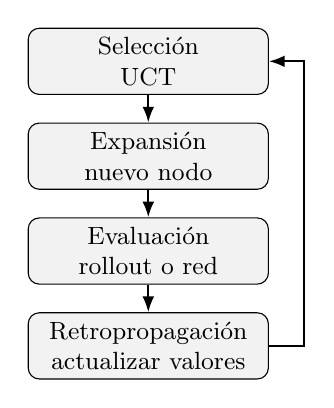
\begin{tikzpicture}[
  node distance=0.35cm,
  phase/.style={draw, rounded corners, align=center, minimum width=3.05cm,
    minimum height=0.58cm, fill=gray!10, font=\small},
  arrow/.style={-{Latex[length=2mm]}, thick}
]
\node[phase] (selection) {Selección\\UCT};
\node[phase, below=of selection] (expansion) {Expansión\\nuevo nodo};
\node[phase, below=of expansion] (evaluation) {Evaluación\\rollout o red};
\node[phase, below=of evaluation] (backprop) {Retropropagación\\actualizar valores};
\draw[arrow] (selection) -- (expansion);
\draw[arrow] (expansion) -- (evaluation);
\draw[arrow] (evaluation) -- (backprop);
\draw[arrow] (backprop.east) -- ++(0.45,0) |- (selection.east);
\end{tikzpicture}
\caption{Fases principales de una iteración de MCTS con UCT.}
\label{fig:fases-uct}
\end{figure}

\subsection{Red neuronal de valor}

La red neuronal resuelve una tarea de regresión supervisada. La entrada contiene
128 atributos: un canal binario para las fichas propias y otro canal binario
para las fichas rivales. La salida es un número real en \([-1, 1]\), obtenido con
una activación \texttt{tanh}. El valor objetivo es \(+1\) si el jugador activo en
ese estado ganó la partida, \(0\) si empató y \(-1\) si perdió.

Aunque el enunciado menciona herramientas como TensorFlow, la red se ha
implementado con NumPy para mantener el proyecto ligero y completamente
ejecutable en el entorno disponible. La arquitectura usada en el experimento
final tiene dos capas ocultas densas de 64 y 32 neuronas, activación ReLU en las
capas ocultas y activación \texttt{tanh} en la salida. El entrenamiento usa error
cuadrático medio y descenso de gradiente por mini-lotes mediante
retropropagación.

\begin{table}[h]
\centering
\caption{Arquitectura de la red de valor.}
\label{tab:red}
\begin{tabular}{lll}
\toprule
Capa & Tamaño & Activación \\
\midrule
Entrada & 128 & -- \\
Oculta 1 & 64 & ReLU \\
Oculta 2 & 32 & ReLU \\
Salida & 1 & tanh \\
\bottomrule
\end{tabular}
\end{table}

\begin{figure}[t]
\centering
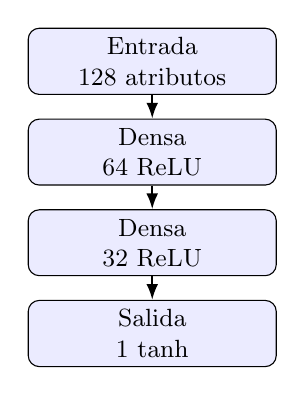
\begin{tikzpicture}[
  node distance=0.3cm,
  layer/.style={draw, rounded corners, align=center, minimum width=3.15cm,
    minimum height=0.58cm, fill=blue!8, font=\small},
  arrow/.style={-{Latex[length=2mm]}, thick}
]
\node[layer] (input) {Entrada\\128 atributos};
\node[layer, below=of input] (h1) {Densa\\64 ReLU};
\node[layer, below=of h1] (h2) {Densa\\32 ReLU};
\node[layer, below=of h2] (output) {Salida\\1 tanh};
\draw[arrow] (input) -- (h1);
\draw[arrow] (h1) -- (h2);
\draw[arrow] (h2) -- (output);
\end{tikzpicture}
\caption{Esquema de la red neuronal de valor utilizada.}
\label{fig:red-valor}
\end{figure}

El valor predicho no debe interpretarse como una probabilidad calibrada en
sentido estadístico estricto, sino como una estimación normalizada de ventaja
para el jugador activo. Valores cercanos a \(1\) indican posiciones que la red
considera favorables, valores cercanos a \(-1\) posiciones desfavorables y
valores próximos a \(0\) posiciones equilibradas o inciertas.

\subsection{Trabajo relacionado}

La búsqueda adversaria clásica, incluyendo minimax y poda alfa-beta, se estudia
habitualmente como punto de partida para juegos deterministas de dos jugadores
con información perfecta~\cite{russell2020}. Estos métodos exploran el árbol de
juego de manera sistemática, pero necesitan funciones heurísticas cuando no es
posible llegar hasta estados terminales. En Otelo, como en ajedrez o Go, la
profundidad completa de la partida hace inviable una expansión exhaustiva en
tiempo real.

MCTS ofrece una alternativa más flexible porque concentra el esfuerzo en las
ramas que parecen más prometedoras según la experiencia acumulada durante las
simulaciones. El artículo de Browne et al.~\cite{browne2012} resume variantes
de MCTS y presenta UCT como una forma efectiva de resolver el dilema entre
explorar acciones poco probadas y explotar acciones con buenos resultados
previos. Esta idea encaja bien con juegos como Otelo, donde el factor de
ramificación cambia mucho a lo largo de la partida.

Los trabajos de AlphaGo y AlphaZero muestran que las redes neuronales pueden
mejorar la búsqueda cuando aprenden a evaluar posiciones o a priorizar
movimientos~\cite{silver2016, silver2017}. La propuesta desarrollada aquí no
pretende reproducir esos sistemas, que usan arquitecturas profundas, grandes
cantidades de cómputo y entrenamiento iterativo. La contribución de este trabajo
es una versión reducida y explicable: UCT proporciona la búsqueda y una red de
valor sencilla sustituye la simulación aleatoria de la política por defecto.

\section{Implementación}

El proyecto se organiza como un paquete Python. El módulo \texttt{game.py}
implementa las reglas, \texttt{mcts.py} implementa UCT, \texttt{agents.py}
define los jugadores, \texttt{self\_play.py} genera datasets,
\texttt{neural.py} define la red de valor, \texttt{train.py} lanza el
entrenamiento a partir de un dataset guardado y \texttt{tournament.py} ejecuta
comparativas. Además, \texttt{cli.py} proporciona los comandos de juego y
\texttt{web\_gui.py} implementa la interfaz gráfica local en navegador.

\subsection{Motor del juego}

El motor del juego se implementa en la clase \texttt{OthelloState}. Cada estado
contiene el tablero, el jugador activo y el número de pases consecutivos. Esta
última variable permite detectar correctamente el final de la partida cuando
ambos jugadores pasan. Los estados se tratan como objetos inmutables: al aplicar
una jugada se crea un nuevo estado con un tablero copiado. Esta decisión aumenta
el coste de memoria, pero simplifica la búsqueda porque los nodos del árbol no
comparten tableros modificables.

El módulo también incluye funciones auxiliares para convertir coordenadas de
texto, calcular puntuaciones, representar el tablero en ASCII y obtener
características para la red. La versión final incorpora una interfaz gráfica
local en navegador, implementada con un servidor HTTP de la biblioteca estándar
de Python. Esta interfaz permite hacer clic en las casillas legales y ver la
respuesta del agente sin introducir coordenadas manualmente.

\subsection{Interfaz gráfica}

La interfaz gráfica se implementa en \texttt{web\_gui.py} sin dependencias
externas adicionales. El servidor local expone una página HTML y varios
endpoints JSON para consultar el estado de la partida, aplicar una jugada
humana, ejecutar el movimiento de la máquina y comenzar una nueva partida. Esta
decisión mantiene el proyecto ligero y evita depender de bibliotecas gráficas
que pueden no estar instaladas en todos los equipos.

El tablero se muestra como una cuadrícula \(8 \times 8\) con las fichas negras y
blancas. Las casillas legales aparecen resaltadas y el usuario puede seleccionar
la jugada mediante un clic. Tras cada movimiento humano se introduce una pausa
breve antes de la respuesta de la máquina, de modo que se pueda observar el
estado intermedio y no parezca que ambos movimientos se han producido al mismo
tiempo. Cuando la partida termina, la interfaz muestra una ventana emergente con
el ganador, el marcador final y la opción de iniciar otra partida.

La interfaz también permite elegir el rival antes de comenzar una partida. Se
puede jugar contra los agentes de referencia, como \texttt{random},
\texttt{greedy} o \texttt{heuristic}, contra UCT con distinto número de
iteraciones o contra UCTNN usando el modelo entrenado. De esta forma, la misma
herramienta sirve tanto para probar manualmente el comportamiento del motor como
para enseñar durante la defensa la diferencia entre un agente UCT clásico y un
agente UCT que utiliza la red neuronal como función de valor. La ejecución por
consola se conserva mediante \texttt{python3 -m othello\_ai.cli --text}.

\subsection{Agentes implementados}

Se han implementado varios agentes para disponer de rivales de dificultad
creciente. El agente aleatorio elige uniformemente una acción legal y sirve como
baseline mínimo. El agente voraz selecciona la jugada que voltea más fichas en
el movimiento inmediato. El agente heurístico combina diferencia de fichas,
movilidad y esquinas. Finalmente, los agentes UCT y UCTNN usan búsqueda de árbol
con la diferencia de que UCTNN recibe una red neuronal entrenada como evaluador.

Disponer de estos agentes facilita el análisis experimental. Si el agente UCT no
superase al aleatorio o al voraz, probablemente habría un error en la búsqueda o
en las reglas. Si UCTNN no mejorase a los baselines, la causa podría estar en la
calidad del dataset, en la arquitectura de la red o en la integración con MCTS.

El agente heurístico no forma parte del requisito principal de junio, pero se
incluyó para disponer de una referencia intermedia entre el agente voraz y UCT.
Su evaluación combina tres criterios. La diferencia de fichas mide la ventaja
material actual; la movilidad mide cuántas acciones legales conserva cada
jugador; y las esquinas capturan un aspecto estratégico importante, ya que una
ficha situada en una esquina no puede ser volteada posteriormente. La ponderación
usada no se ha optimizado automáticamente, sino que se ha elegido como una
heurística simple y explicable.

Esta variedad de agentes también permite detectar comportamientos anómalos. Por
ejemplo, un agente que gana al aleatorio pero pierde claramente contra el voraz
puede estar tomando decisiones localmente razonables pero estratégicamente
débiles. Un agente que mejora al voraz pero no escala al aumentar iteraciones
puede estar limitado por la política por defecto. Estas comparaciones son
importantes porque una única partida aislada no permite evaluar de forma fiable
la calidad de un jugador.

\subsection{Integración de la red en UCT}

La integración se realiza mediante un parámetro \texttt{evaluator} en la clase
\texttt{UCTSearch}. Si este parámetro es nulo, la evaluación de un nodo no
terminal se obtiene mediante la política por defecto, que realiza una simulación
hasta el final de la partida o hasta un límite de profundidad. Si el parámetro
contiene una función, UCT llama directamente a esa función y limita el resultado
al intervalo \([-1,1]\). El agente UCTNN pasa como evaluador una llamada a
\texttt{network.predict\_state}.

Esta decisión evita duplicar el código de MCTS: el mismo algoritmo sirve para la
versión clásica y para la versión neuronal. La diferencia de comportamiento
queda localizada en la función de evaluación, que es precisamente el punto que
pide modificar el enunciado de la convocatoria de junio.

\begin{figure*}[t]
\begin{pseudo}*
\hd{\fn{UCT}}(estado, iters) \\*
\textbf{Entrada}: estado actual del juego \\
\textbf{Salida}: movimiento seleccionado \\
raiz \(\leftarrow\) nuevo nodo con estado \\
repetir \(iters\) veces \\+
  nodo \(\leftarrow\) \fn{selección}(raiz) \\
  si nodo no es terminal entonces \\+
    nodo \(\leftarrow\) \fn{expandir}(nodo) \\-
  valor \(\leftarrow\) \fn{eval}(nodo.estado) \\
  \fn{backprop}(nodo, valor) \\-
devolver mejor hijo de raiz
\end{pseudo}
\caption{Esquema del algoritmo UCT implementado.}
\label{pcd:uct}
\end{figure*}

La política por defecto de la versión básica realiza una simulación aleatoria
hasta final de partida. La versión con red neuronal sustituye esa simulación por
una llamada al modelo de valor, reduciendo el coste de evaluación y guiando la
búsqueda hacia posiciones aprendidas mediante autojuego.

\subsection{Generación de datos}

El dataset se genera mediante partidas automáticas entre dos copias del mismo
agente. Durante cada partida se guardan los estados intermedios después de cada
movimiento. Al finalizar, cada estado recibe como etiqueta el resultado de la
partida desde la perspectiva del jugador activo en ese estado. De esta forma, el
mismo tablero puede tener interpretaciones distintas si cambia el jugador al que
le toca mover.

Para aumentar el número de ejemplos se aplican las ocho simetrías del tablero:
cuatro rotaciones y sus reflejos horizontales. Estas transformaciones conservan
el resultado estratégico de la posición, por lo que permiten aumentar el dataset
sin generar nuevas partidas. En el experimento final, 50 partidas de autojuego
produjeron 23792 ejemplos tras aplicar estas simetrías.

\subsection{Entrenamiento de la red}

El entrenamiento se separa en dos niveles. El módulo \texttt{neural.py} contiene
la implementación de la red neuronal, incluyendo propagación hacia delante,
cálculo de la pérdida, retropropagación y guardado/carga de pesos. El módulo
\texttt{train.py} actúa como punto de entrada desde consola: carga el archivo
\texttt{npz} generado por autojuego, construye una \texttt{ValueNetwork} con las
capas indicadas por argumentos, ejecuta el entrenamiento durante el número de
épocas elegido y guarda el modelo entrenado en \texttt{models/}.

Esta separación permite reutilizar la red desde otros módulos sin repetir código
de entrenamiento. Por ejemplo, \texttt{experiments.py} usa directamente
\texttt{ValueNetwork} para automatizar todo el pipeline, mientras que
\texttt{train.py} permite entrenar manualmente un modelo concreto cambiando
parámetros como capas ocultas, tasa de aprendizaje, tamaño de lote o número de
épocas.

\begin{figure*}[t]
\centering
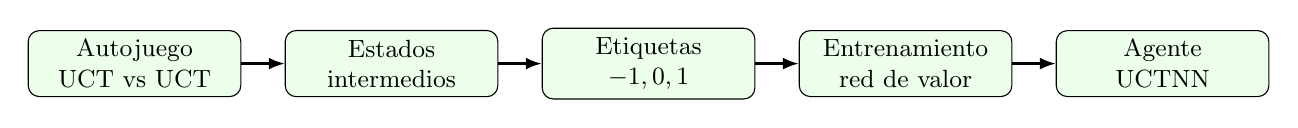
\begin{tikzpicture}[
  node distance=0.55cm,
  block/.style={draw, rounded corners, align=center, minimum width=2.7cm,
    minimum height=0.75cm, fill=green!8, font=\small},
  arrow/.style={-{Latex[length=2mm]}, thick}
]
\node[block] (selfplay) {Autojuego\\UCT vs UCT};
\node[block, right=of selfplay] (states) {Estados\\intermedios};
\node[block, right=of states] (labels) {Etiquetas\\$-1,0,1$};
\node[block, right=of labels] (training) {Entrenamiento\\red de valor};
\node[block, right=of training] (agent) {Agente\\UCTNN};
\draw[arrow] (selfplay) -- (states);
\draw[arrow] (states) -- (labels);
\draw[arrow] (labels) -- (training);
\draw[arrow] (training) -- (agent);
\end{tikzpicture}
\caption{Flujo completo de generación de datos, entrenamiento y uso del modelo.}
\label{fig:flujo-experimental}
\end{figure*}

\subsection{Reproducibilidad}

Los experimentos se agrupan en el módulo \texttt{experiments.py}. Este script
genera el dataset, entrena la red, ejecuta los torneos y escribe los resultados
en formato Markdown y JSON. Además, todas las llamadas usan semillas
configurables. Esto permite repetir la misma ejecución durante la defensa o
modificar fácilmente el número de partidas, épocas o iteraciones UCT.

\begin{table}[h]
\centering
\caption{Artefactos principales generados por el proyecto.}
\label{tab:artefactos}
\begin{tabular}{ll}
\toprule
Fichero & Contenido \\
\midrule
\texttt{selfplay\_experiment.npz} & Dataset de estados y etiquetas \\
\texttt{value\_net\_experiment.npz} & Pesos de la red entrenada \\
\texttt{experiment\_results.md} & Resumen legible de torneos \\
\texttt{experiment\_results.json} & Resultados estructurados \\
\texttt{memoria-otelo.pdf} & Documento final compilado \\
\bottomrule
\end{tabular}
\end{table}

Los ficheros \texttt{npz} se han elegido porque permiten almacenar varios
arrays NumPy comprimidos en un único archivo. El dataset contiene los atributos
\texttt{x}, las etiquetas \texttt{y} y metadatos sobre el agente usado para el
autojuego. El modelo contiene el tamaño de entrada, las capas ocultas y las
matrices de pesos y sesgos de cada capa. Esta separación permite regenerar el
modelo desde cero o reutilizar uno ya entrenado en torneos posteriores.

\subsection{Coste computacional}

El coste de una decisión UCT depende principalmente del número de iteraciones y
del coste de evaluar cada nodo expandido. En la versión básica, cada evaluación
puede implicar una simulación completa de partida. Aunque Otelo tiene un tablero
pequeño, una simulación puede contener decenas de movimientos y cada movimiento
requiere volver a calcular acciones legales. Por ello, aumentar el número de
iteraciones mejora la calidad de la búsqueda, pero también incrementa
rápidamente el tiempo por jugada.

La versión neuronal modifica este equilibrio. Evaluar una posición con la red
consiste en varias multiplicaciones matriciales pequeñas: \(128 \times 64\),
\(64 \times 32\) y \(32 \times 1\). Este coste es mucho más estable que una
simulación aleatoria completa. La desventaja es que la evaluación deja de ser
una muestra directa del resultado de una partida y pasa a depender de la calidad
del entrenamiento. En otras palabras, UCT básico suele ser más caro pero menos
sesgado por el dataset; UCTNN es más rápido, pero puede equivocarse
sistemáticamente si la red ha aprendido mal ciertas posiciones.

\begin{table}[h]
\centering
\caption{Comparación cualitativa de evaluadores dentro de UCT.}
\label{tab:evaluadores}
\begin{tabular}{lll}
\toprule
Evaluador & Ventaja & Riesgo \\
\midrule
Rollout & No requiere datos & Coste alto y ruido \\
Heurística & Muy rápido & Diseño manual \\
Red valor & Rápido y aprendido & Depende del dataset \\
\bottomrule
\end{tabular}
\end{table}

En los resultados obtenidos se aprecia esta diferencia. El torneo UCT-16 contra
Greedy tardó 36.4 segundos, mientras que UCTNN-16 contra Greedy tardó 2.5
segundos. La comparación no mide solo una jugada, pero sí muestra que sustituir
rollouts por una red reduce mucho el tiempo total de juego. La cuestión abierta
es mejorar la calidad del evaluador neuronal para que esa ganancia de velocidad
no implique perder fuerza de juego.

\section{Pruebas y experimentación}

Se han preparado pruebas unitarias para verificar los movimientos legales
iniciales, el volteo de fichas, la obligación de pasar, la detección de final de
partida y la integración básica de UCT. Estas pruebas se ejecutan con:

\begin{verbatim}
python3 -m unittest discover -s tests -v
\end{verbatim}

En la ejecución realizada se superaron 8 pruebas unitarias. Estas pruebas no
demuestran que el agente sea óptimo, pero sí reducen el riesgo de fallos
básicos en el motor: movimientos iniciales incorrectos, volteos mal aplicados,
pases ilegales o partidas que no terminan. También se verifica que UCT siempre
devuelve una acción legal en el estado inicial y que la red puede realizar al
menos una iteración de entrenamiento.

\subsection{Diseño experimental}

Los torneos alternan el color inicial entre agentes para reducir el sesgo de que
negras muevan primero. La medida principal es el número de victorias, derrotas y
empates. Como medida secundaria se usa la diferencia media de fichas desde la
perspectiva del agente A, porque permite distinguir victorias ajustadas de
victorias amplias. También se registra el tiempo total de cada torneo para
comparar el coste de los distintos evaluadores.

El experimento reproducible se ejecutó con el siguiente comando:

\begin{verbatim}
python3 -m othello_ai.experiments \
  --selfplay-games 50 \
  --selfplay-agent uct:12 \
  --epochs 35 \
  --tournament-games 12 \
  --uct-iters 16 \
  --seed 23
\end{verbatim}

La configuración se eligió como compromiso entre tiempo de ejecución y
capacidad de obtener resultados interpretables en un entorno local. Frente a una
primera prueba con 12 partidas, se aumentó el autojuego a 50 partidas para que
la red recibiera posiciones más variadas. Los resultados siguen sin ser una
estimación definitiva de fuerza de juego, pero ya permiten valorar mejor el
efecto de usar una función de valor aprendida.

\begin{table}[h]
\centering
\caption{Configuración y resultado del entrenamiento.}
\label{tab:entrenamiento}
\begin{tabular}{lr}
\toprule
Magnitud & Valor \\
\midrule
Partidas de autojuego & 50 \\
Agente de autojuego & UCT-12 \\
Ejemplos generados & 23792 \\
Capas ocultas & 64, 32 \\
Épocas & 35 \\
Loss entrenamiento & 0.79606 \\
Loss validación & 0.80524 \\
\bottomrule
\end{tabular}
\end{table}

El conjunto de entrenamiento se generó por autojuego usando UCT con 12
iteraciones por decisión. Cada estado intermedio se etiquetó con el resultado
final desde la perspectiva del jugador activo y se aplicaron las ocho simetrías
del tablero. La pérdida de validación bajó de 0.91996 a 0.80524, lo que indica
que la red aprende una señal útil y mejora claramente respecto a la prueba
inicial con menos partidas.

\begin{table*}[t]
\centering
\caption{Resultados de los torneos. La diferencia media se mide desde la perspectiva del agente A.}
\label{tab:torneos}
\begin{tabular}{llrrrrr}
\toprule
Agente A & Agente B & Partidas & Victorias A & Victorias B & Empates & Dif. media A \\
\midrule
Greedy & Random & 12 & 9 & 3 & 0 & 8.83 \\
Heurístico & Greedy & 12 & 11 & 1 & 0 & 24.92 \\
UCT-16 & Greedy & 12 & 8 & 4 & 0 & 6.00 \\
UCT-32 & UCT-16 & 12 & 7 & 4 & 1 & 9.33 \\
UCTNN-16 & Random & 12 & 11 & 0 & 1 & 17.33 \\
UCTNN-16 & Greedy & 12 & 9 & 3 & 0 & 9.50 \\
UCTNN-16 & UCT-16 & 12 & 10 & 2 & 0 & 13.33 \\
\bottomrule
\end{tabular}
\end{table*}

La tabla~\ref{tab:torneos} muestra tres conclusiones principales. En primer
lugar, las heurísticas simples ya son claramente superiores al jugador aleatorio,
por lo que son buenos rivales de control. En segundo lugar, UCT mejora al jugador
voraz incluso con solo 16 iteraciones, y aumentar a 32 iteraciones produce una
mejora frente a UCT-16. En tercer lugar, UCTNN-16 obtiene los mejores resultados
del experimento ampliado: gana 11 partidas y empata una contra Random, supera
9--3 a Greedy y vence 10--2 a UCT-16. Este cambio respecto a la prueba inicial
muestra que aumentar el dataset tuvo un efecto positivo en la utilidad de la red.

También se observa una diferencia clara de coste temporal. El torneo UCT-16
contra Greedy tardó 36.4 segundos, mientras que el torneo UCTNN-16 contra Greedy
tardó 2.5 segundos. Esta diferencia aparece porque la red sustituye las
simulaciones aleatorias completas de la política por defecto por una evaluación
directa del estado.

\subsection{Análisis de errores y limitaciones}

El resultado más importante desde el punto de vista crítico es que UCTNN-16
mejora claramente tras ampliar el dataset. En la prueba inicial, entrenada con
solo 12 partidas, no superaba al agente voraz. Con 50 partidas de autojuego y
23792 ejemplos tras simetrías, el mismo enfoque vence a Greedy y a UCT-16. Esto
apoya la hipótesis de que la función de valor aprendida depende mucho de la
cantidad y variedad de estados usados durante el entrenamiento.

Otra limitación es que la red predice solo el valor del estado, no una política
de movimientos. Esto significa que UCTNN sigue expandiendo acciones sin una guía
neuronal directa sobre qué jugadas son más prometedoras. En sistemas como
AlphaZero se aprenden simultáneamente una política y una función de valor, lo
que permite dirigir mucho mejor la búsqueda. En este trabajo se ha mantenido una
versión más sencilla porque el objetivo de la convocatoria es reemplazar la
política por defecto de UCT por una red de evaluación.

Por último, el número de partidas de torneo es bajo. Doce partidas por
emparejamiento permiten observar tendencias, pero no proporcionan una estimación
estadística estable. Para una evaluación más fuerte sería conveniente repetir
los torneos con al menos 50 o 100 partidas por enfrentamiento y varias semillas
distintas.

\subsection{Amenazas a la validez}

La primera amenaza a la validez interna es la aleatoriedad. MCTS, los agentes
aleatorios y la inicialización de la red dependen de semillas. Aunque los
experimentos fijan una semilla para poder reproducir los resultados, otras
semillas podrían producir variaciones, especialmente con tan pocas partidas. Por
ese motivo, las conclusiones se formulan como tendencias observadas y no como
afirmaciones absolutas sobre la fuerza de cada agente.

La segunda amenaza es el sesgo del generador de datos. Como el autojuego se
realizó con un agente UCT pequeño, las posiciones del dataset reflejan el estilo
de juego y los errores de ese agente. Si se generasen partidas con más
iteraciones, con varios tipos de rivales o mediante reentrenamiento iterativo,
la red probablemente recibiría ejemplos más variados y podría mejorar su
capacidad de generalización.

La tercera amenaza es la escala del entrenamiento. Aunque el dataset ampliado es
más razonable que el inicial, sigue siendo pequeño comparado con los enfoques de
aprendizaje por autojuego a gran escala. Esta decisión fue adecuada para mantener
el proyecto ejecutable en un ordenador personal, pero limita la calidad máxima
del evaluador neuronal. Aún así, el experimento es suficiente para comprobar el
requisito principal de la convocatoria: diseñar una red, entrenarla con estados
de Otelo y usarla dentro de MCTS como reemplazo de la política por defecto.

\subsection{Uso del proyecto}

El proyecto está preparado para poder mostrar tres tipos de ejecución. La
primera es una partida interactiva contra la máquina usando la interfaz gráfica
en navegador. Esta ejecución permite comprobar que el motor aplica las reglas
correctamente y que el agente devuelve movimientos legales. La segunda es un
torneo corto entre dos agentes, útil para mostrar cómo se comparan los jugadores
sin intervención humana. La tercera es la ejecución del script de experimentos,
que reproduce el pipeline completo de generación de datos, entrenamiento y
evaluación.

\section{Conclusiones}

El proyecto implementa el pipeline completo solicitado para la convocatoria de
junio: reglas de Otelo, UCT, generación de estados por autojuego, entrenamiento
de una red neuronal y uso de esa red como evaluador dentro de la búsqueda. La
principal ventaja del enfoque es que separa claramente el motor del juego, la
búsqueda y el aprendizaje.

Los resultados muestran que UCT es una mejora sólida sobre los baselines simples
y que la red neuronal aprende una función de valor con información útil. Con el
dataset ampliado, el agente UCTNN-16 supera a Random, Greedy y UCT-16 en los
torneos realizados. La interpretación más plausible es que aumentar la cantidad
de autojuego mejora la calidad del evaluador neuronal y permite que la red aporte
una ventaja real dentro de MCTS.

Como trabajo futuro se propone aumentar el número de partidas de entrenamiento,
comparar distintas arquitecturas de red, ajustar la constante de exploración de
UCT y realizar reentrenamiento iterativo. También sería posible aprender una
política de movimientos además de la función de valor, acercando el sistema a
los enfoques usados en AlphaZero.

\begin{thebibliography}{00}
\bibitem{russell2020} S. Russell and P. Norvig, \emph{Artificial Intelligence:
A Modern Approach}, 4th ed. Pearson, 2020.
\bibitem{browne2012} C. B. Browne et al., ``A survey of Monte Carlo Tree Search
methods,'' \emph{IEEE Transactions on Computational Intelligence and AI in
Games}, vol. 4, no. 1, pp. 1--43, 2012.
\bibitem{silver2016} D. Silver et al., ``Mastering the game of Go with deep
neural networks and tree search,'' \emph{Nature}, vol. 529, pp. 484--489, 2016.
\bibitem{silver2017} D. Silver et al., ``Mastering Chess and Shogi by self-play
with a general reinforcement learning algorithm,'' arXiv:1712.01815, 2017.
\end{thebibliography}

\end{document}
